\selectlanguage{ngerman}
\thispagestyle{empty}
{\vrule height 0mm depth 30mm width 0mm}
%\vspace*{2em}
\par\noindent 
\uppercase{Textgestaltung}\par\vspace{1.0ex}
\noindent Bei der Textgestaltung werden die Grundsätze befolgt, die in den Vorworten zu den Bänden I,~5 und VI,~6 als für alle Reihen verbindlich festgelegt wurden. Dabei gilt insbesondere:\par
1. Jedes unbetitelte Stück erhält eine Überschrift in der Sprache des Stückes. Eigene Überschriften von Leibniz werden übernommen, jedoch hinsichtlich der Groß- und Kleinschreibung sowie der Akzentuierungen den anderen Überschriften angepasst. Das Leibniz'sche Original wird unmittelbar vor dem Text wiederholt.\par
2. Die Groß- und Kleinschreibung lateinischer Texte wird gemäß den Editionen der Klassiker normalisiert. Insbesondere werden i und j sowie u und v entsprechend vereinheitlicht. Vollständige Sätze werden mit einem Punkt abgeschlossen. Jeder Satzanfang wird groß geschrieben. Akzente fallen weg.\par
3. In französischen Texten wird das Schriftbild beibehalten, jedoch werden Akzente dort ergänzt, wo Missverständnisse entstehen können. Fehlt bei Leibniz offensichtlich ein Apostroph, so ergänzen wir es. Wenn ein \glqq que\grqq\ als Kürzel auftritt, wird es im modernen Sinne aufgelöst. Sprachliche Versehen werden verbessert, wenn Leibniz die richtige Form zur fraglichen Zeit kennt und verwendet (Beispiel: \glqq certaines corps\grqq\ statt \glqq certains corps\grqq\ bei Leibniz wird verbessert). Sie werden beibehalten, wenn Leibniz die falsche Form vorsätzlich, etwa auf Grund einer Änderung, niederschreibt (Beispiel: contante), seine Kenntnis der richtigen Form also nicht sicher belegt ist.\par
4. Die Leibniz'sche Interpunktion wird bewahrt. Hinzugefügte Zeichen werden, abgesehen von den unter Punkt 2 und 3 genannten Fällen sowie bei offensichtlichen Flüchtigkeiten, in eckige Klammern gesetzt.\par
\par\vspace{5.0ex}
%\clearpage
\noindent\uppercase{Variantengestaltung}\par\vspace{1.0ex}
\noindent
Die Variantengestaltung erfolgt gemäß den Regeln der anderen Reihen. Eine Variante ist durch Zeilenangabe sowie vorderen und hinteren Anschluss eindeutig mit dem Haupttext verknüpft.
Streichungen und Ergänzungen werden zwischen senkrechte Striche gesetzt;
Ergänzungen können auch durch bloße Angabe des hinzugefügten Textes dargestellt werden.
Bei Ersetzungen kennzeichnen vorangestellte Ziffern \textit{(1)}, \textit{(2)}, \textit{(3)} ... und Buchstaben \textit{(a)}, \textit{(b)}, \textit{(c)} ..., \textit{(aa)}, \textit{(bb)}, \textit{(cc)} ... die Stufen der Gedankenentwicklung. Jede nachfolgende Stufe hebt die vorhergehende auf. Nachgestellte Siglen (in diesem Band meist \textit{L}) bezeichnen den Textzeugen, welchem die Variante entnommen ist. Um bei tief gestuften Varianten die Übersicht zu wahren, werden die Bezeichnungen zu Fünfergruppen zusammengefasst und wie folgt wiedergegeben: \textit{(aaaaa-a)} ... \textit{(bbbbb-b)} ... \textit{(aaaaa-aa)} ... \textit{(bbbbb-bb)} usw. Treten innerhalb von Varianten Ergänzungen und Streichungen auf, die ihrerseits wieder Varianten enthalten, so werden solche Streichungen und Ergänzungen als eigenständige Textteile behandelt. Die Variantenzählung beginnt in diesen Fällen neu.\par
In den Varianten werden Wortlaut, Zeichensetzung und Rechnungen grundsätzlich nicht berichtigt, auch nicht bei offensichtlichen Fehlern. Abbrechende Wörter werden nicht vervollständigt. Die letzte Korrekturstufe kann aus Platzgründen abgekürzt wiedergegeben werden. Die Auslassungen werden durch Punkte in eckigen Klammern kenntlich gemacht.\par\vspace{2.0ex}
%\clearpage
\noindent Beispieltext zur Variantengestaltung nach VIII,~1 N.~21\textsubscript{2}\par\vspace{1.0ex}
\noindent{\scriptsize21}\hspace{5mm}polito, quam rugoso tapete decurrat. Sed quam precaria quantisque difficulta-\newline %
{\scriptsize22}\hspace{5mm}tibus obsita sit haec Hypothesis quam aliena similitudine confirmata dudum a\newline
{\scriptsize23}\hspace{5mm}multis observatum est.\par\vspace{0.5cm}
\noindent \footnotesize 21\textendash 23\enskip decurrat. \textit{(1)}~Sed \textit{(a)}~quam obscura \textit{(b)}~quam obnoxia difficultatibus \textit{(c)}~quis concedat \textit{(aa)}~omne rar \textit{(bb)}~quantum unum quodque corpus est, rarius tanto esse villo. \textit{(2)}~Sed \textit{(a)}~quantis difficultati \textit{(b)}~quam [...] Hypothesis \textbar\ quam aliena similitudine \textit{(1)}~adhibita \textit{(2)}~confirmata; dudum \textit{erg.}\ \textbar\ a multis \textit{(aa)}~expositum est \textit{(aaa)}~vero \textit{(bbb)}~et ausim dicere vix \textit{(bb)}~observatum est. \textit{L}\par
\vspace{1.0ex}	
\noindent 21\textendash 23\enskip decurrat.\par\noindent
\hspace{7mm}\textit{(1)}\ Sed\par\noindent
\hspace{14mm}\textit{(a)}\ quam obscura\par\noindent
\hspace{14mm}\textit{(b)}\ quam obnoxia difficultatibus\par\noindent
\hspace{14mm}\textit{(c)}\ quis concedat\par\noindent
\hspace{21mm}\textit{(aa)}\ omne rar\par\noindent
\hspace{21mm}\textit{(bb)}\ quantum unum quodque corpus est, rarius tanto esse villo.\par\noindent
\hspace{7mm}\textit{(2)}\ Sed\par\noindent
\hspace{14mm}\textit{(a)}\ quantis difficultati\par\noindent
\hspace{14mm}\textit{(b)}\ quam \lbrack...\rbrack\ Hypothesis \textbar\ quam aliena similitudine \textit{(1)} adhibita\par\noindent
\hspace{8.25cm}\textit{(2)}\ confirmata; dudum \textit{erg.} \textbar\ a
multis\par\noindent
\hspace{21mm}\textit{(aa)}\ expositum est\par\noindent
\hspace{29mm}\textit{(aaa)} vero\par\noindent
\hspace{29mm}\textit{(bbb)} et ausim dicere vix\par\noindent
\hspace{21mm}\textit{(bb)} observatum est. \textit{L}
\par
%\vspace{5.0ex}
\newpage%%%
\normalsize
%%%%%%%%%%%Anfang:  Kollationen %%%%%%%%%%%%%%
\noindent\uppercase{Kollationen}\par\vspace{1.0ex}
\noindent
Ist ein Stück durch mehr als einen Textzeugen überliefert (\textit{L}, \textit{l}, \textit{Lil}, \textit{E}, \textit{LiE}), erfolgt eine Kollation (in diesem Band N.~\ref{cnds_3}, N.~\ref{ddrs_06}, N.~\ref{adva_2}): Einer dieser Zeugen wird als Grundlage für den Haupttext des edierten Stückes herangezogen und als \glqq Unsere Druckvorlage\grqq\ in der  \glqqÜberlieferung\grqq\ ausgewiesen. Für alle Stellen, an denen die Zeugen mit der Druckvorlage und untereinander übereinstimmen, also keine Abweichungen im gültigen Text oder der Textgenese aufweisen, bleibt der Apparat stumm. Weichen die Zeugen hinsichtlich des gültigen Texts oder dessen Genese von der Druckvorlage oder voneinander ab, werden ihre Varianten im textkritischen Apparat angegeben, und zwar mit jeweils eigenem vorderem Anschlusswort und mit der Sigle des zitierten Zeugen (oder mit den Siglen der Zeugen, falls mehrere dieselbe Variante aufweisen). Eine mit diesen Varianten einhergehende Textgenese wird gemäß der oben beschriebenen Variantengestaltung dokumentiert. Der textkritische Apparat kann darüber hinaus bei Kollationen je nach Vorkommen folgende Phänomene vermerken (teils mit eigenen Formulierungen):
\par
\vspace{6pt}
\noindent\textemdash\ Zeugen überliefern den im Apparat angeführten (ggf. durch \lbrack...\rbrack\ gekürzten) Text der Druckvorlage nicht (\textit{fehlt}), z.\,B.:\par %Bsp. aus 14.6
{\footnotesize%
4\textendash S.~239.8\hspace{5mm}Scientia Mechanica \lbrack...\rbrack\ unice desideratur. \textit{fehlt~L\textsuperscript{3}}
}%%%
\par
\vspace{6pt}
\noindent\textemdash\ Der im Apparat angeführte Text eines Zeugen ist als gestrichen bzw. ungültig zu werten (\textit{versehentlich erhalten}), z.\,B.:\par%\vspace{2pt} %Bsp. aus 12.3
{\footnotesize%
11\hspace{5mm}monuimus. \lbrack2v\textsuperscript{o}\rbrack\
\textit{(1)}~Sed
\textit{(2)}~Hic
\textbar~ergo \textit{erg.}~%
\textbar\ distinctius
\textbar~cognosci \textit{versehentlich erhalten}~\textbar\ }%%%
\par\vspace{-3pt}
{\footnotesize explicari meretur
\textbar~editum \textit{erg.}~% ~L\textsuperscript{1}, fehlt~l
\textbar\ admirandae%
~\textit{L\textsuperscript{1}}
}%%%
\par
\vspace{6pt}
\noindent\textemdash\ Gestrichener Text eines Zeugen ist als nicht gestrichen bzw. gültig zu werten (\textit{versehentlich gestr.}).
\par
\noindent\textemdash\ Zeugen haben eine von der Druckvorlage oder voneinander abweichende Zeichensetzung, die der Apparat nach dem Anschlusswort durch ein zusätzliches Leerzeichen besonders kenntlich macht, z.\,B.:\par %Bsp. aus 14.6
{\footnotesize%
4\hspace{5mm}partes~,~\textit{L\textsuperscript{1}}\quad
partes\,~\textit{L\textsuperscript{2}}\quad
partes~,~\textit{E\textsuperscript{1}}
}%%%
\par
\vspace{6pt}
\noindent\textemdash\ Zeugen heben, abweichend von der Druckvorlage oder voneinander, Text hervor oder nicht, z.\,B.:\par %Bsp. aus 14.6
{\footnotesize%
4\hspace{5mm}in \hspace{0,5mm} fig.~1%
~\textit{L\textsuperscript{1}}\quad
\hspace{0,5mm}\textso{in} \textso{fig.}~\textso{1}%
~\textit{L\textsuperscript{2}}%
}%%%
\par 
\vspace{3.0ex}
%%%%%%%%%%%Ende:  Kollationen %%%%%%%%%%%%%%
%
%\clearpage
\newpage
\noindent\uppercase{Rechnungen und Notation}\par\vspace{1.0ex}
\noindent Die Leibniz'sche mathematische Notation wird durch Kursivierung verein\-heitlicht. Nebenrechnungen werden wie Marginalien behandelt und direkt unter den Text gesetzt. Leibniz benutzt die zu seiner Zeit übliche Überwärtsdivision mit ihren charakteristischen Streichungen und rechnet gelegentlich \glqq fortlaufend\grqq\ weiter, d.h. er verwendet bei Gleichungsketten Zwischenergebnisse ohne Neuansatz (vgl. VIII,~1 N.~36).\par
%\vspace{-0.2mm}
\begin{center}
$\begin{array}{lllr}             
\hspace{5.5pt}\cancel{3}2&&&\\
\hspace{5.5pt}\cancel{7}\cancel{8}&&&\\
\cancel{2}\cancel{3}\cancel{6}2&&\hspace{11pt}2644&\\
\cancel{7}\cancel{2}\cancel{2}\cancel{5}&f&\hspace{16.5pt}147&\\
\cancel{4}\cancel{9}\cancel{9}\cancel{9}&&\overline{\hspace{5.5pt}18508}&\\
\hspace{5.5pt}\cancel{4}\cancel{4}&&10576&\\
  &&2644&\\
  &&\overline{388668}&
 \end{array}$  
\end{center}
Zu den Besonderheiten der Rechentechnik gehört weiterhin, dass Leibniz zur Vermeidung von Fallunterscheidungen Doppelvorzeichen verwendet, die paarweise oder auch mehrfach zusammengesetzt sein können. Darüber hinaus benutzt er neben den auch heute üblichen runden Klammern ein- bzw. zweiseitige Halbklammern, die im Text durch Kommata bzw. $\llcorner$  und $\lrcorner$ wiedergegeben werden (vgl. VIII,~1 N.~54).\par
%  \def\leibdashvv{\diatop[$\vspace{10pt}-$|$|$]}
%                     \def\leibdashv{\diatop[$\leibdashvv$|$\hspace{-5.15pt}\dashv$]}
%                    \def\leibvdash{\protect\raisebox{10.5pt}{\protect\scalebox{1}[-1]{$\leibdashv$}}}      
                    \begin{center}
$\protect\begin{array}{rl}\displaystyle \leibdashv \hspace{5pt} x \hspace{5pt} \leibvdash \hspace{5pt} \displaystyle\protect\frac{\beta^2}{2} &\protect\sqcap\hspace{5pt} \protect\sqrt{ \protect\llcorner \displaystyle\protect\frac{1}{4} - 2 \protect\lrcorner \beta^2,, + \protect\llcorner 4 - \displaystyle\protect\frac{1}{2}a \protect\lrcorner \displaystyle\protect\frac{a^3\beta}{n^2},, + \protect\llcorner8 - \displaystyle\protect\frac{1}{8}\protect\lrcorner \protect\frac{a^6}{n^4}}\vspace{0.1cm}\\ \displaystyle\protect\frac{4a^3}{n^2}&\protect\end{array}$
\end{center}
Aus Gründen der Vereinfachung von Gleichungen und Termen markiert Leibniz einzelne Rechenschritte durch Streichungen oder abgerundete Umrahmungen, und er bezeichnet in mehrzeiligen Schemata mehrfach auftretende Formelbestandteile durch Punktierung (vgl. VIII,~1 N.~54).
\begin{center}
   $\begin{array}{r}\displaystyle z^4- 8ax\hspace{3pt}z^2\\+4a\beta ..\\\rule[0cm]{0cm}{20pt}
                               \end{array}
                               \Bigg\{\begin{array}{ll}\displaystyle+64a^2x^2&\sqcap\\\displaystyle-64a^2\beta x&\\\displaystyle \frac{+16a^2\beta^2}{4}&\end{array}
                     \begin{array}{ll}\displaystyle+8a^2x^2&\\\displaystyle-8a^2\beta x&\\\displaystyle \ovalbox{$+4a^2\beta^2\hspace{-35pt}\raisebox{-13pt}{$-4a^2\beta^2$}$}&\end{array}$
\end{center}
\newpage
\par
%\par\vspace{5.0ex}
\noindent\uppercase{Besonderheiten bei Figuren und Zeichnungen}\par\vspace{1.0ex}
\noindent
Figuren und Zeichnungen wurden von Leibniz in der Regel in Tinte aus\-geführt. Nicht ungewöhnlich sind auch Zeichnungen, die teilweise als Blind\-zeichnungen überliefert sind. Seltener treten Bleistiftzeichnungen auf. Die Blind\-zeichnungen werden von den übrigen durch Aufhellung unterschieden. Sie erscheinen daher im Druckbild grau.\par
Sämtliche Figuren und Zeichnungen werden für den Fall, dass Leibniz sie nicht bezeichnet hat, stückbezogen durchnummeriert. Die vom Editor hinzugefügten Bezeichnungen werden in eckige Klammern gesetzt und kursiviert.\par
Die Notation innerhalb von Zeichnungen wird mit der des Schriftbefunds abgeglichen und kursiv wiedergegeben. Dabei werden Groß- und Kleinschreibung harmonisiert. Fehlende oder inkorrekte Notationen innerhalb von Zeichnungen werden in eckigen Klammern hinzugefügt bzw.\ geändert und in den Erläuterungen kommentiert.\par
%%Die Figuren und Zeichnungen aus den Marginalienexemplaren wurden dem Original folgend nachgezeichnet. Dadurch kann es zu Abweichungen in der Strich\-stärke sowie hinsichtlich der Kursivierung der Bezeichnungen kommen. In diesen Exemplaren hat Leibniz häufig Elemente von Zeichnungen durch Zusätze versehen. Für den Fall, dass es sich dabei um Bezeichnungen handelt, werden diese Zusätze durch runde kursivierte Klammern kenntlich gemacht.
%%%\clearpage
Beispiel einer Zeichnung mit Blindzeichnung und nachträglich vom Editor hinzugefügten Elementen aus VIII,~1 N.~13\textsubscript{4}: 
\begin{center}
  \includegraphics[trim = 0mm 0mm 0mm -15mm, clip,width=0.65\textwidth]{images/38_21v.pdf}
\end{center}
%%\newpage
%%Beispiel einer Zeichnung aus I. Barrows \textit{Lectiones opticae}, in die Leibniz nachträglich Bezeichnungen eingefügt hat VIII,~1 N.~26:
%%\begin{center}
%%    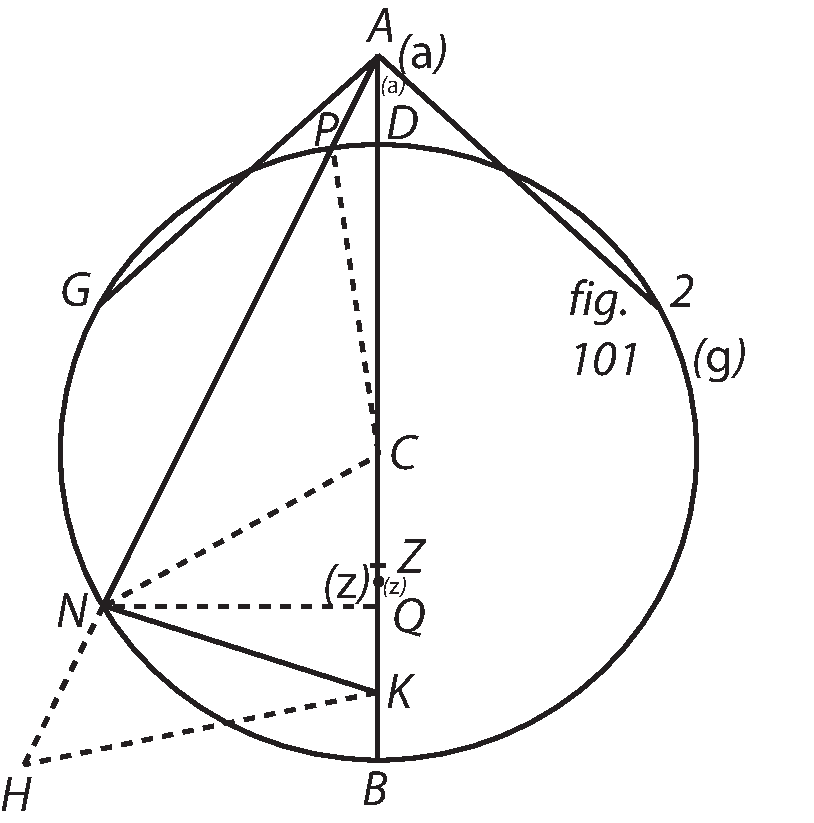
\includegraphics[trim = 0mm 0mm 0mm -5mm, clip,width=0.4\textwidth]{images/T8_Barrow-2.pdf}
%%\end{center}
\clearpage